\documentclass[10pt]{article}
\usepackage[utf8]{inputenc}
\usepackage[T1]{fontenc}
\usepackage{amsmath}
\usepackage{amsfonts}
\usepackage{amssymb}
\usepackage[version=4]{mhchem}
\usepackage{stmaryrd}
\usepackage{bbold}
\usepackage{graphicx}
\usepackage[export]{adjustbox}
\graphicspath{ {./images/} }

\begin{document}
\section*{Lecture hours 24-26}
\section*{Definitions and Theorems}
Definition ( Transpose of a matrix Matrix).\\
The transpose of a matrix $A$ is $A^{T}$, and it has columns the rows of A (same order).

Definition ( Perpendicular complement).\\
Let $V$ be a subspace of $\mathbb{R}^{n}$, then $W$ is called the "perpendicular complement" of $V$ and denoted $V^{\perp}$ (pronounced "V perp", symbol $\perp$ is a superscript ) if $W$ contains all vector in $\mathbb{R}^{n}$ that are perpendicular to all vectors in $V$.

Definition (Fundamental subspaces of linear algebra).\\
For any m by n matrix $A$ we have\\
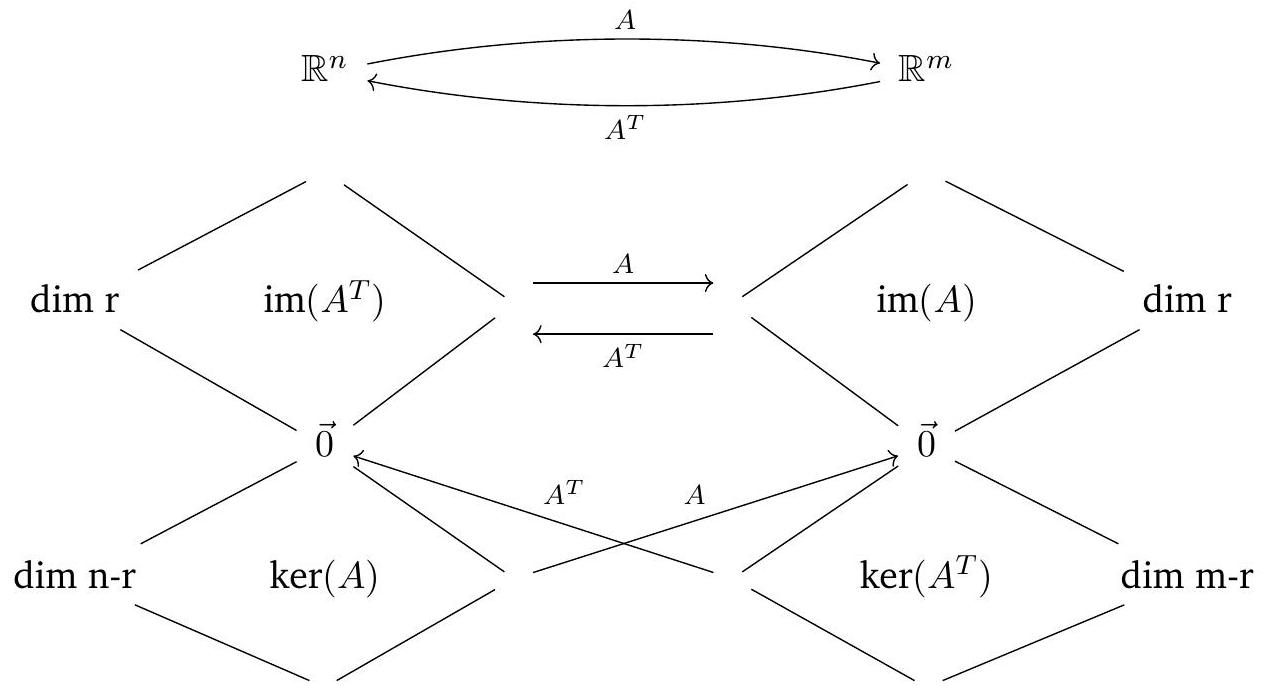
\includegraphics[max width=\textwidth, center]{2024_12_26_a34900bcde57bec02ea9g-1}

$$
(\operatorname{ker} A)^{\perp}=\operatorname{im}\left(A^{T}\right), \quad(\operatorname{im} A)^{\perp}=\operatorname{ker}\left(A^{T}\right)
$$

Problem 43 (Fundamental subspaces of linear algebra). Consider the matrix

$$
A=\left[\begin{array}{cc}
2 & 1 \\
-1 & 0 \\
0 & 0
\end{array}\right]
$$

Find $\operatorname{ker}(A), \operatorname{im}(A), \operatorname{ker}\left(A^{T}\right)$, and $\operatorname{im}\left(A^{T}\right)$. For each of these subspaces, determine the value of $n$ for which they are a subspace of $\mathbb{R}^{n}$.

Solution 43 (Fundamental subspaces of linear algebra) $\operatorname{ker}(A)=\{\overrightarrow{0}\} \subset \mathbb{R}^{2}, \operatorname{im}(A)=$ $\operatorname{span}\left(\vec{e}_{1}, \vec{e}_{2}\right) \subset \mathbb{R}^{3}, \operatorname{ker}\left(A^{T}\right)=\operatorname{span}\left(\vec{e}_{3}\right) \subset \mathbb{R}^{3}$, and $\operatorname{im}\left(A^{T}\right)=\mathbb{R}^{2}$.\\
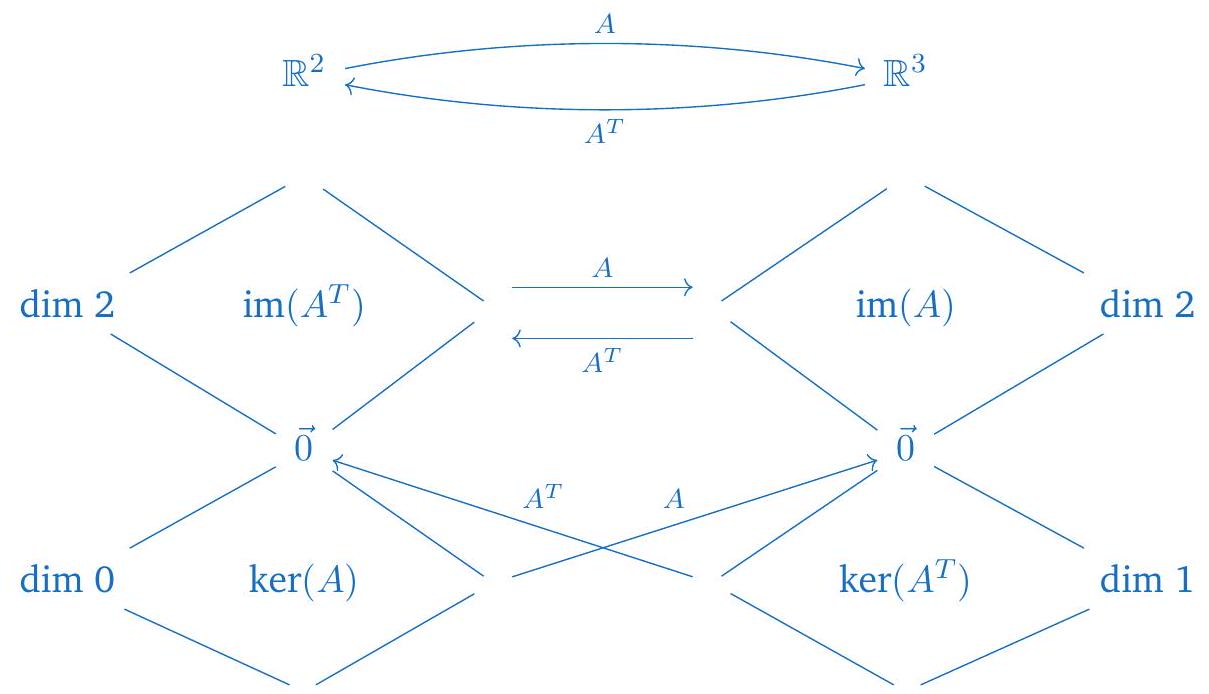
\includegraphics[max width=\textwidth, center]{2024_12_26_a34900bcde57bec02ea9g-2}

Problem 44 (Transpose of a matrix). Let $A$ be an invertible $n \times n$ matrix.\\
a) Explain why $A^{T}$ is invertible.\\
b) Explain why $\left(A^{T}\right)^{-1}=\left(A^{-1}\right)^{T}$. (Hint: $I^{T}=I$.)

Solution 44 (Transpose of a matrix)\\
a) $A^{T}$ is square, so to show that is invertible it is sufficient to show that $\operatorname{ker}\left(A^{T}\right)=$ $\{\overrightarrow{0}\}$. We know that $A$ is invertible, so $\operatorname{im}(A)=\mathbb{R}^{n}$. We always have $\operatorname{im}(A)^{\perp}=$ $\operatorname{ker}\left(A^{T}\right)$, and $\left(\mathbb{R}^{n}\right)^{\perp}=\{\overrightarrow{0}\}$, so we do indeed have $\operatorname{ker}\left(A^{T}\right)=\{\overrightarrow{0}\}$.\\
b) We have the formula $A^{-1} A=I$. Transposing both sides gives $A^{T}\left(A^{-1}\right)^{T}=I$. Similarly, transposing both sides of $A A^{-1}=I$ gives $\left(A^{-1}\right)^{T} A^{T}=I$.Therefore, the inverse matrix of $A^{T}$ is $\left(A^{-1}\right)^{T}$.

Problem 45 (Least squares - Normal Equations). You are given data points $(x, y)=$ $(1,1),(2,3),(-1,3)$. Use a least squares line of best fit to predict the $y$-value when $x=7$.

Solution 45 (Least squares - Normal Equations) From fitting a line $y=m x+c$ to the given data points we get equations:

$$
\left[\begin{array}{cc}
1 & 1 \\
2 & 1 \\
-1 & 1
\end{array}\right]\left[\begin{array}{l}
m \\
c
\end{array}\right]=\left[\begin{array}{l}
1 \\
3 \\
3
\end{array}\right]
$$

We can solve this use the method of normal equations.

Let

$$
\vec{x}^{*}=\left[\begin{array}{c}
m \\
c
\end{array}\right], \quad A=\left[\begin{array}{cc}
1 & 1 \\
2 & 1 \\
-1 & 1
\end{array}\right] \quad \text { and } \quad \vec{b}=\left[\begin{array}{l}
1 \\
3 \\
3
\end{array}\right]
$$

We know $\vec{x}^{*}$ is a least squares solution of

$$
A \vec{x}^{*}=\vec{b}
$$

if and only if $\vec{b}-A \vec{x}^{*} \in(\operatorname{Im} A)^{\perp}$ (take a look at figure below).\\
But we have seen that $(\operatorname{Im} A)^{\perp}=\operatorname{ker}\left(A^{T}\right)$, so we $\vec{x}^{*}$ such that

$$
A^{T}\left(\vec{b}-A \vec{x}^{*}\right)=\overrightarrow{0}
$$

Solving for $\vec{x}^{*}$ we obtain that

$$
\begin{gathered}
\vec{x}^{*}=\left(A^{T} A\right)^{-1} A^{T} \vec{b} \\
A^{T} A=\left[\begin{array}{ll}
6 & 2 \\
2 & 3
\end{array}\right], \quad\left(A^{T} A\right)^{-1}=\frac{1}{14}\left[\begin{array}{cc}
3 & -2 \\
-2 & 6
\end{array}\right], \quad A^{T} \vec{b}=\left[\begin{array}{l}
4 \\
7
\end{array}\right] .
\end{gathered}
$$

Putting this together, our least squares solution has $m=-1 / 7, c=17 / 7$. Therefore, when $x=7$, we predict $y=10 / 7$.\\
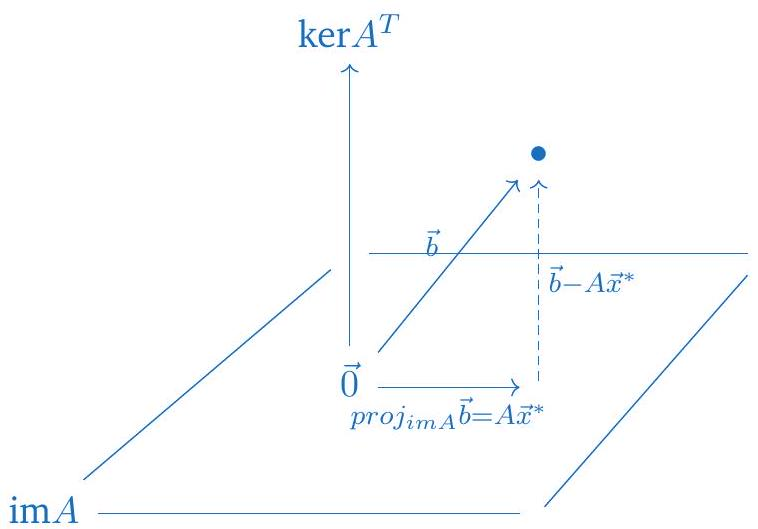
\includegraphics[max width=\textwidth, center]{2024_12_26_a34900bcde57bec02ea9g-4}


\end{document}